\documentclass[conference]{IEEEtran}

\usepackage[utf8]{inputenc}
\usepackage{amsmath,amssymb}
\usepackage{graphicx}
\usepackage{booktabs}
\usepackage{tabularx}
\usepackage{xcolor}
\usepackage{hyperref}
\usepackage{enumitem}
\graphicspath{{figures/}{report/figures/}{./}}

% Hyperlink configuration
\hypersetup{
    colorlinks=true,
    linkcolor=teal!80!black,
    citecolor=blue!70!black,
    urlcolor=blue!70!black
}

\title{From Symptoms to Decisions: Deciphering Clinical Complexity, Diagnostic Overlap, and Dataset Imbalance in Medical Records\\
\large Course: 23CSE353 --- Data Visualization | Problem Code: MED-04}

\author{
    \IEEEauthorblockN{Athirasree A S}
    \IEEEauthorblockA{
        \vspace{0.1cm}
        Dept. of Computer Science and Engineering\\
        Amrita School of Computing, Bengaluru\\
        Amrita Vishwa Vidyapeetham, India\\
        Email: bl.sc.u4cse24205@bl.students.amrita.edu
    }
}

\begin{document}

\maketitle

\begin{abstract}
Electronic Health Record (EHR) triage systems face persistent operational challenges balancing intake survey duration against diagnostic discrimination. This case study analyzes a 4,920-record clinical benchmark spanning 131 symptoms and 41 diseases to empower hospital triage directors and health analytics teams to make informed structural decisions. Adhering to the \textit{Action-Target-Purpose} (ATP) framework, we conduct rigorous exploratory data profiling, uncovering critical synthetic anomalies including a zero-variance duplicate header bug (\texttt{fluid\_overload}), an artificial class balance of exactly 120 cases per disease, and high permutation redundancy. We formulate five analytical questions prior to graphical design and answer each with perceptually grounded visualizations. Key empirical findings reveal: (1) an extreme bimodal symptom specificity spectrum where 61.1\% of symptoms are pathognomonic anchors while only two symptoms (\textit{fatigue} and \textit{vomiting}) span over 41\% of conditions; (2) a four-fold disparity in patient symptom burden ranging from 4 symptoms in acute cardiac/urinary events to 17 symptoms in multi-system viral infections; (3) severe diagnostic ambiguity zones exceeding 80\% cosine overlap among viral hepatitis variants and 63--67\% between malaria/typhoid and pneumonia/tuberculosis; and (4) an extreme Pareto symptom distribution where the top 20 symptoms generate >50\% of all clinical mentions, while 66 symptoms account for 80\%. Based on these findings, we propose a modular two-stage dynamic intake triage architecture and automated laboratory reflex safety rails. Complete reproducible workflows for Tableau dashboards and Jupyter notebooks are provided.
\end{abstract}

\begin{IEEEkeywords}
Clinical Informatics, Outpatient Triage, Exploratory Data Analysis, Diagnostic Ambiguity, Tableau Visual Analytics, Dataset Imbalance.
\end{IEEEkeywords}

\section{Introduction \& Clinical Problem Statement}
In contemporary healthcare systems, outpatient triage and emergency room intake represent the critical initial touchpoint between presenting patients and clinical care pathways~\cite{gilboy2011emergency}. With the increasing adoption of digital patient intake portals and clinical decision support systems (CDSS), healthcare providers frequently rely on standardized symptom questionnaires. However, poorly calibrated questionnaires create two operational pathologies:
\begin{enumerate}[noitemsep]
    \item \textbf{Questionnaire Fatigue \& Intake Latency:} Administering extensive, non-adaptive symptom lists causes patient drop-off and delays urgent triage assignments.
    \item \textbf{Diagnostic Ambiguity \& False-Certainty:} Subjective symptom reports frequently fail to distinguish between conditions sharing high clinical overlap, exposing triage systems to misclassification risks when laboratory confirmation is omitted~\cite{cabitza2017unintended}.
\end{enumerate}

Under problem statement \textbf{MED-04: Symptoms to Disease}, a health analytics team seeks to understand the global topology of medical symptom records: determining which symptoms are universally shared, which diseases possess near-identical symptom profiles, and where the dataset exhibits structural imbalances. Crucially, the objective of this investigation is \textit{not} to construct an automated diagnostic algorithm, but rather to communicate patterns, structural risks, and clinical insights clearly to institutional decision-makers.

\begin{table*}[t]
\centering
\small
\caption{The Action-Target-Purpose (ATP) Decision Framework for Problem MED-04.}
\label{tab:atp}
\begin{tabularx}{\textwidth}{l p{4.2cm} X}
\toprule
\textbf{Dimension} & \textbf{Core Question} & \textbf{Operational Implementation} \\
\midrule
\textbf{ACTION} & What specific action or decision should this analysis support? & 
1. Transition static 131-item intake questionnaires into dynamic, two-stage branching triage protocols.\newline
2. Establish mandatory automated laboratory reflex orders for disease pairs exhibiting high symptom overlap ($\ge 0.60$ cosine similarity).\newline
3. Recalibrate clinical machine learning pipelines to correct for synthetic class balance and dead-feature artifacts prior to hospital deployment. \\
\addlinespace
\textbf{TARGET} & Who is the primary audience and decision-maker? & 
\textbf{Health Analytics Director, Clinical Informatics Operations Committee, and Emergency Department Triage Protocol Leads.} \\
\addlinespace
\textbf{PURPOSE} & Why does this decision matter to the organization? & 
1. \textbf{Projected Latency Reduction:} Targets an estimated $\sim 60\%$ intake questionnaire time reduction by replacing exhaustive 131-item checklists with dynamic 2-stage branching protocols.\newline
2. \textbf{Prevents Diagnostic Harm:} Halts premature symptom-only discharge for ambiguous conditions (e.g., Viral Hepatitis or Malaria vs. Typhoid).\newline
3. \textbf{Prevents Algorithmic Failure:} Prevents deploying overfitted models trained on synthetic benchmarks that fail in epidemiologically skewed real-world cohorts. \\
\bottomrule
\end{tabularx}
\end{table*}

\section{Strategic Framing: The Action-Target-Purpose (ATP) Framework}
To ensure the analytical inquiry is driven by strategic decisions rather than cosmetic graphing, Table~\ref{tab:atp} outlines the formal Action-Target-Purpose (ATP) matrix governing this project.

\section{Exploratory Data Analysis (EDA) \& Forensic Data Profiling}
Prior to visual encoding, we conducted a rigorous data audit on the 4,920 patient records. This audit uncovered several critical structural anomalies and data engineering artifacts:

\subsection{Data Structure \& Dimensionality}
The primary training dataset provided in the Kaggle benchmark is \texttt{train\_disease.csv}, comprising 4,920 rows and 134 columns, accompanied by the independent evaluation split \texttt{test\_disease.csv} (42 rows and 133 columns). In \texttt{train\_disease.csv}, each row corresponds to a single patient encounter, with the initial 132 columns representing binary symptom indicators ($1 = \text{present}$, $0 = \text{absent}$), followed by the categorical target \texttt{prognosis}.

\subsection{Ghost Columns \& Delimiter Inconsistencies}
Column 134, labeled \texttt{Unnamed: 133}, was found to contain 100\% missing values ($4,920$ NaNs). Forensic inspection confirmed this ghost column was generated by a trailing delimiter comma on each line of the raw CSV file. It was cleanly excised from the analytical pipeline.

\subsection{Duplicate Header Bug \& Zero-Variance Artifacts}
A critical data integrity flaw was identified in the symptom feature headers: the presence of two separate columns corresponding to fluid retention:
\begin{itemize}[noitemsep]
    \item \texttt{fluid\_overload}: Exhibited an absolute sum of $0$ across all 4,920 encounters (zero-variance dead feature).
    \item \texttt{fluid\_overload.1}: Auto-indexed by data parsers, contained $114$ active occurrences, all strictly localized to patients diagnosed with \textit{Alcoholic Hepatitis}.
\end{itemize}
This represents a duplicate header collision in the benchmark source. In our preprocessing pipeline, the dead zero-variance column was dropped, and \texttt{fluid\_overload.1} was restored to its canonical clinical label \texttt{fluid\_overload}.

\subsection{Class Balance vs. Permutation Redundancy}
The target variable \texttt{prognosis} contains exactly 41 distinct disease conditions. Remarkably, every single disease contains \textit{exactly 120 records} ($41 \times 120 = 4,920$). This uniform class distribution is an artifact of synthetic data balancing. 
Furthermore, an audit of symptom vectors within each disease group revealed high permutation redundancy: each disease contains only between 5 and 10 unique clinical symptom patterns, repeated 12 to 24 times each across the 120 records.

\subsection{Clinical Domain Standardization}
Typographical errors in clinical labels (e.g., \texttt{'Peptic ulcer diseae'}, \texttt{'Diabetes '}, \texttt{'Osteoarthristis'}) were programmatically resolved. To provide meaningful high-level operational groupings for hospital triage managers, each condition was categorized into one of six core \textbf{Clinical Specialty Domains}:
\begin{enumerate}[noitemsep]
    \item \textit{Hepato-Biliary \& Digestive} (12 conditions, 1,440 encounters)
    \item \textit{Infectious Diseases} (8 conditions, 960 encounters)
    \item \textit{Dermatology \& Allergy} (6 conditions, 720 encounters)
    \item \textit{Endocrinology \& Metabolism} (4 conditions, 480 encounters)
    \item \textit{Cardiovascular \& Renal} (5 conditions, 600 encounters)
    \item \textit{Neurology \& Musculoskeletal} (6 conditions, 720 encounters)
\end{enumerate}

\section{Analytical Formulation: The Five Core Research Questions}
In compliance with academic visualization methodology, each visual artifact was designed to answer a specific, pre-formulated analytical question:
\begin{itemize}[noitemsep]
    \item \textbf{Question 1 (Ubiquity vs. Specificity):} Which symptoms act as non-specific ``chameleons'' spanning multiple disease categories versus ``pathognomonic anchors'' unique to a single condition, and how does this dictate triage questionnaire hierarchy?
    \item \textbf{Question 2 (Disease Complexity \& Symptom Load):} How does patient symptom burden (number of co-manifesting symptoms) vary across clinical conditions, and which disease categories represent high-complexity multi-system syndromes?
    \item \textbf{Question 3 (Diagnostic Ambiguity \& Similarity):} Which disease pairs share severe symptom profile similarity, creating critical operational risks for triage misdirection and diagnostic confusion?
    \item \textbf{Question 4 (Structural Imbalance \& Synthetic Artifacts):} Where does the dataset exhibit structural imbalance---in disease representation versus symptom rarity---and what synthetic artifacts must healthcare analytics teams account for?
    \item \textbf{Question 5 (Syndromic Co-occurrence Clusters):} What functional symptom clusters co-occur most strongly in patient presentations, and how can clinical intake questionnaires be modularized into dynamic triage branches?
\end{itemize}

\section{Visualizations, Empirical Findings \& Design Choices}
Below, we present the visual evidence answering each analytical question, accompanied by explicit defense justifications addressing: \textit{Why this graph? Why this colour? Why this aggregation? What should the reader notice?}

% ------------------------------------------------------------------------------
\subsection{Question 1: Symptom Ubiquity vs. Specificity Spectrum}
\begin{figure*}[t]
    \centering
    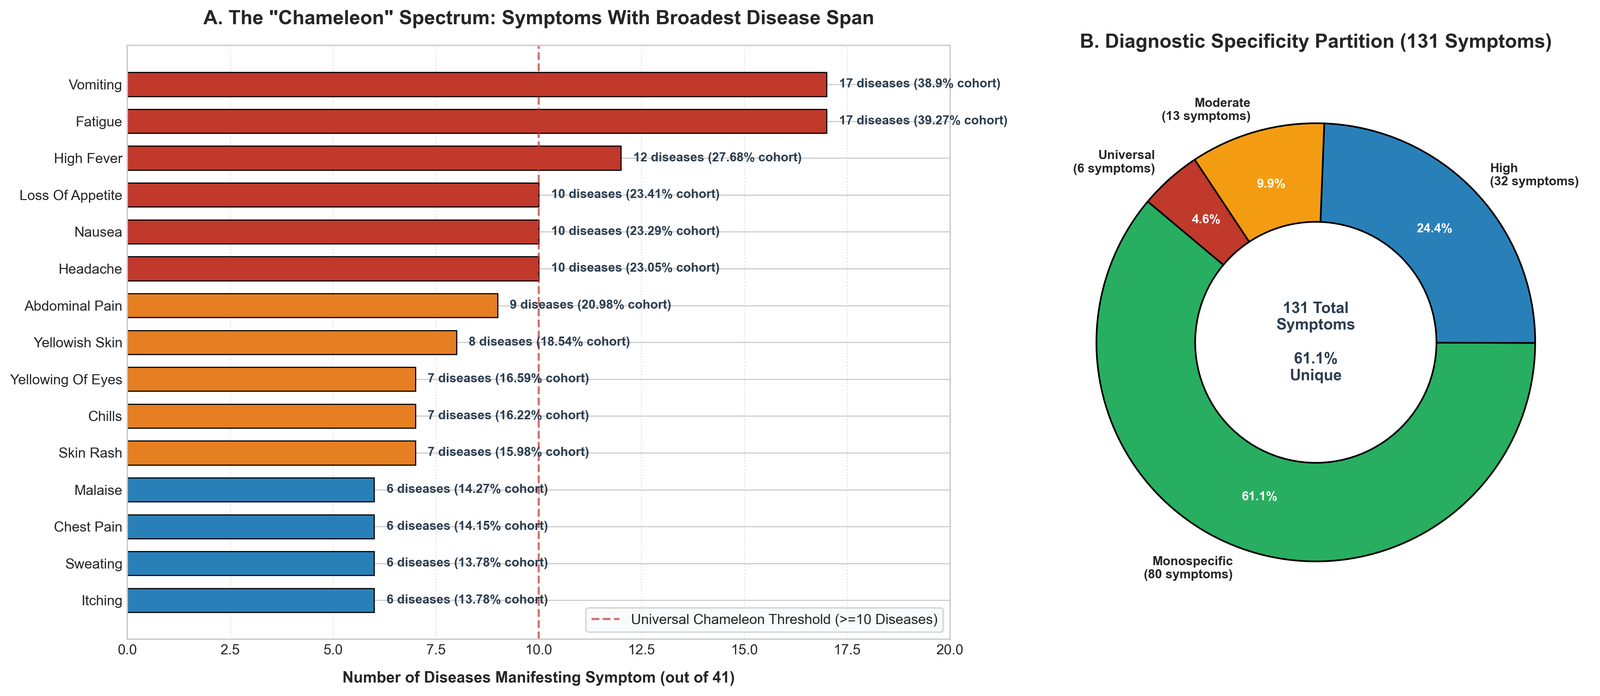
\includegraphics[width=0.92\textwidth]{figures/fig1_symptom_ubiquity_specificity.png}
    \caption{\textbf{Symptom Ubiquity vs. Specificity Spectrum.} Panel A ranks the top 15 most ubiquitous symptoms by disease span and cohort prevalence. Panel B illustrates the four-tier specificity breakdown across all 131 symptoms.}
    \label{fig:q1}
\end{figure*}

\subsubsection{Design Choices (``Explain Your Choices'')}
\begin{itemize}[noitemsep]
    \item \textbf{Why this graph?} A horizontal bar chart facilitates effortless reading of medical terminology without angled text. The complementary donut chart provides a clear part-to-whole partition of diagnostic specificity classes.
    \item \textbf{Why this colour?} A categorical semantic scheme was adopted: high-ambiguity chameleon symptoms ($\ge 10$ diseases) are encoded in warning Crimson (\texttt{\#C0392B}), while high-certainty pathognomonic anchors are encoded in Forest Green (\texttt{\#27AE60}).
    \item \textbf{Why this aggregation?} Feature aggregation uses distinct disease count ($\text{COUNTD}(\text{prognosis})$) and total patient prevalence percentage.
    \item \textbf{What should the reader notice?} The distribution is heavily bimodal: a striking 61.1\% of all symptoms (80 out of 131) are strictly \textit{monospecific} (exclusive to a single disease), whereas a tiny core of symptoms (\textit{fatigue} and \textit{vomiting}, each spanning 17 diseases / 41.5\% of conditions) act as pervasive chameleons.
\end{itemize}

\subsubsection{Clinical Takeaway \& Action}
Triage forms should not present all symptoms uniformly. Stage-1 triage should query the top 10 systemic chameleon symptoms to detect general illness severity, followed immediately by Stage-2 branching to test candidate pathognomonic anchors (e.g., \textit{nodal skin eruptions} for fungal infections, or \textit{throat irritation} for the common cold), confirming a diagnosis in minimal queries.

% ------------------------------------------------------------------------------
\subsection{Question 2: Disease Complexity \& Patient Symptom Burden}
\begin{figure*}[t]
    \centering
    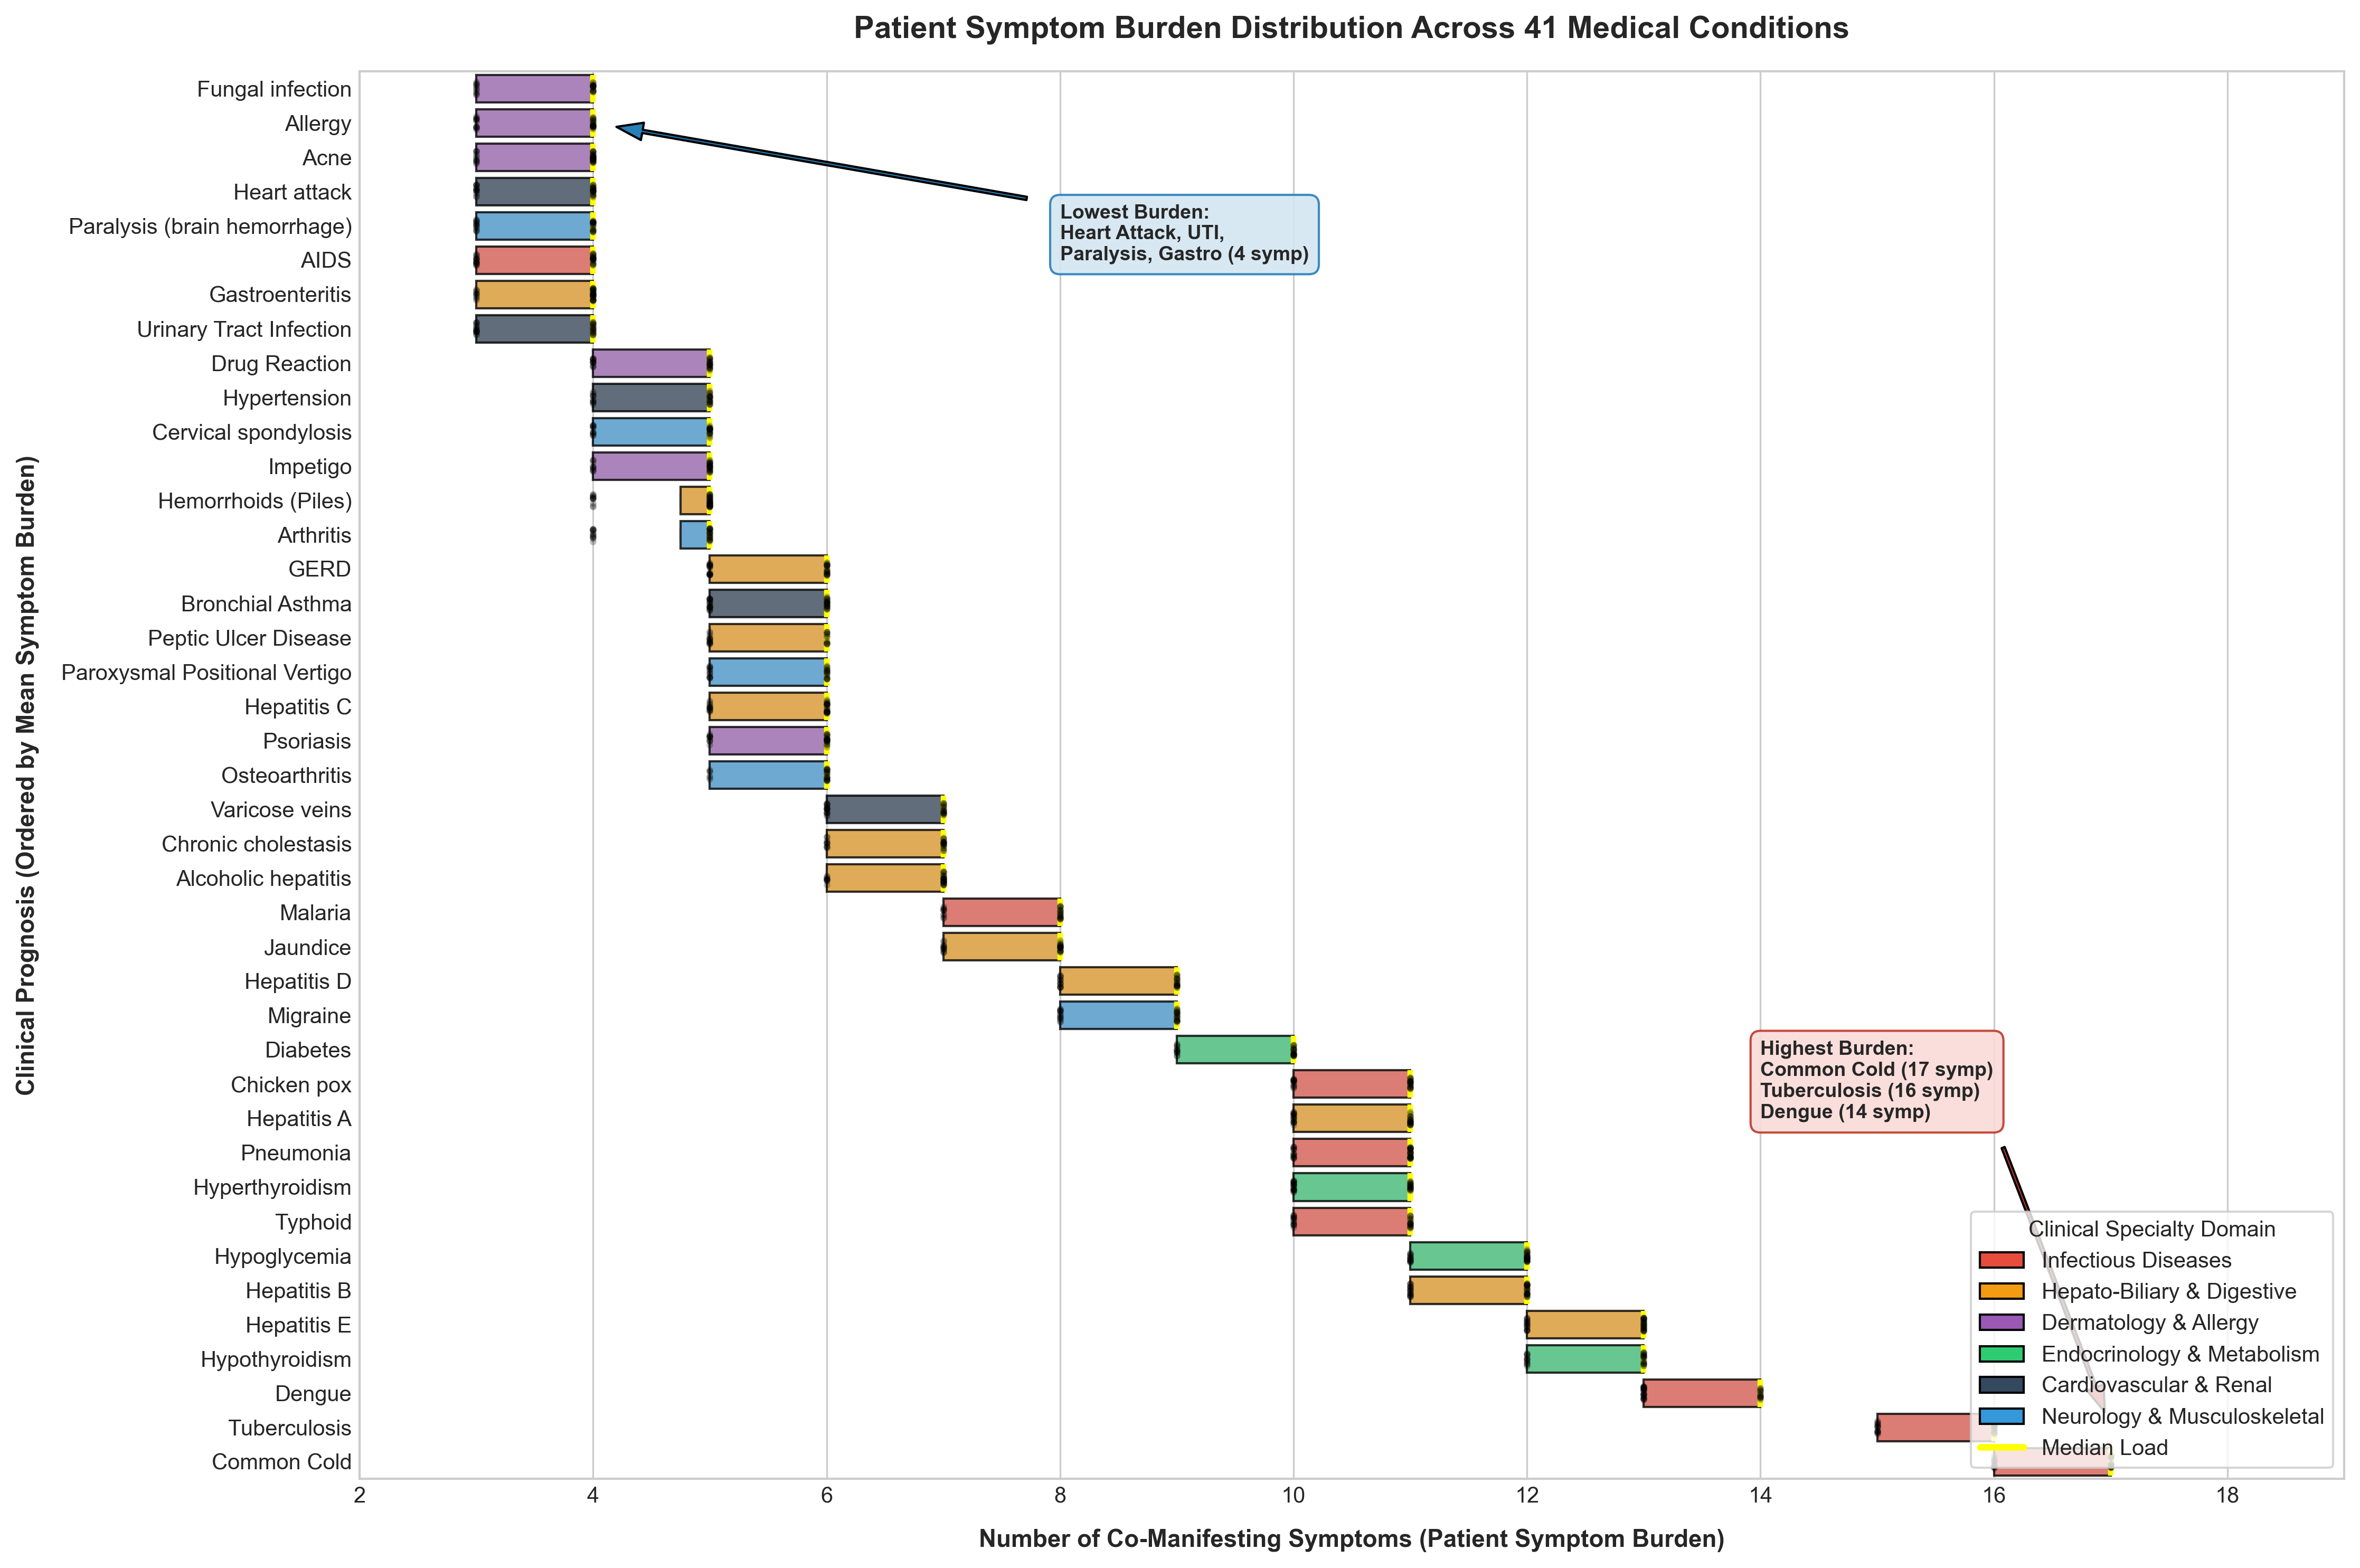
\includegraphics[width=0.90\textwidth]{figures/fig2_disease_complexity_burden.png}
    \caption{\textbf{Patient Symptom Burden Distribution Across 41 Medical Conditions.} Boxplots show median and interquartile range of co-manifesting symptoms, color-coded by Clinical Specialty Domain.}
    \label{fig:q2}
\end{figure*}

\subsubsection{Design Choices (``Explain Your Choices'')}
\begin{itemize}[noitemsep]
    \item \textbf{Why this graph?} An ordered horizontal boxplot with overlaid jittered points visualizes both the central tendency (median/IQR) and discrete patient permutations across all 41 diseases.
    \item \textbf{Why this colour?} Six distinct hues represent hospital clinical specialty departments, enabling instant visual appraisal of domain-level complexity patterns.
    \item \textbf{Why this aggregation?} Row-level summation of active symptoms per encounter, aggregated by Mean, Median, and IQR per disease.
    \item \textbf{What should the reader notice?} A dramatic four-fold disparity exists across clinical conditions: Common Cold ($\bar{x} = 17$ symptoms), Tuberculosis ($\bar{x} = 16$), and Dengue ($\bar{x} = 14$) represent high-burden multi-system infections. In contrast, conditions like Heart Attack, UTI, and Paralysis present with strictly 4 symptoms.
\end{itemize}

\subsubsection{Clinical Takeaway \& Action}
Outpatient clinics must dynamically allocate consultation time slots: high-burden viral/respiratory patients require extended 25-minute slots for multi-system evaluation, whereas low-burden acute presentations require rapid, focused reflex diagnostic pathways.

% ------------------------------------------------------------------------------
\subsection{Question 3: Disease Pairwise Similarity \& Diagnostic Ambiguity}
\begin{figure*}[t]
    \centering
    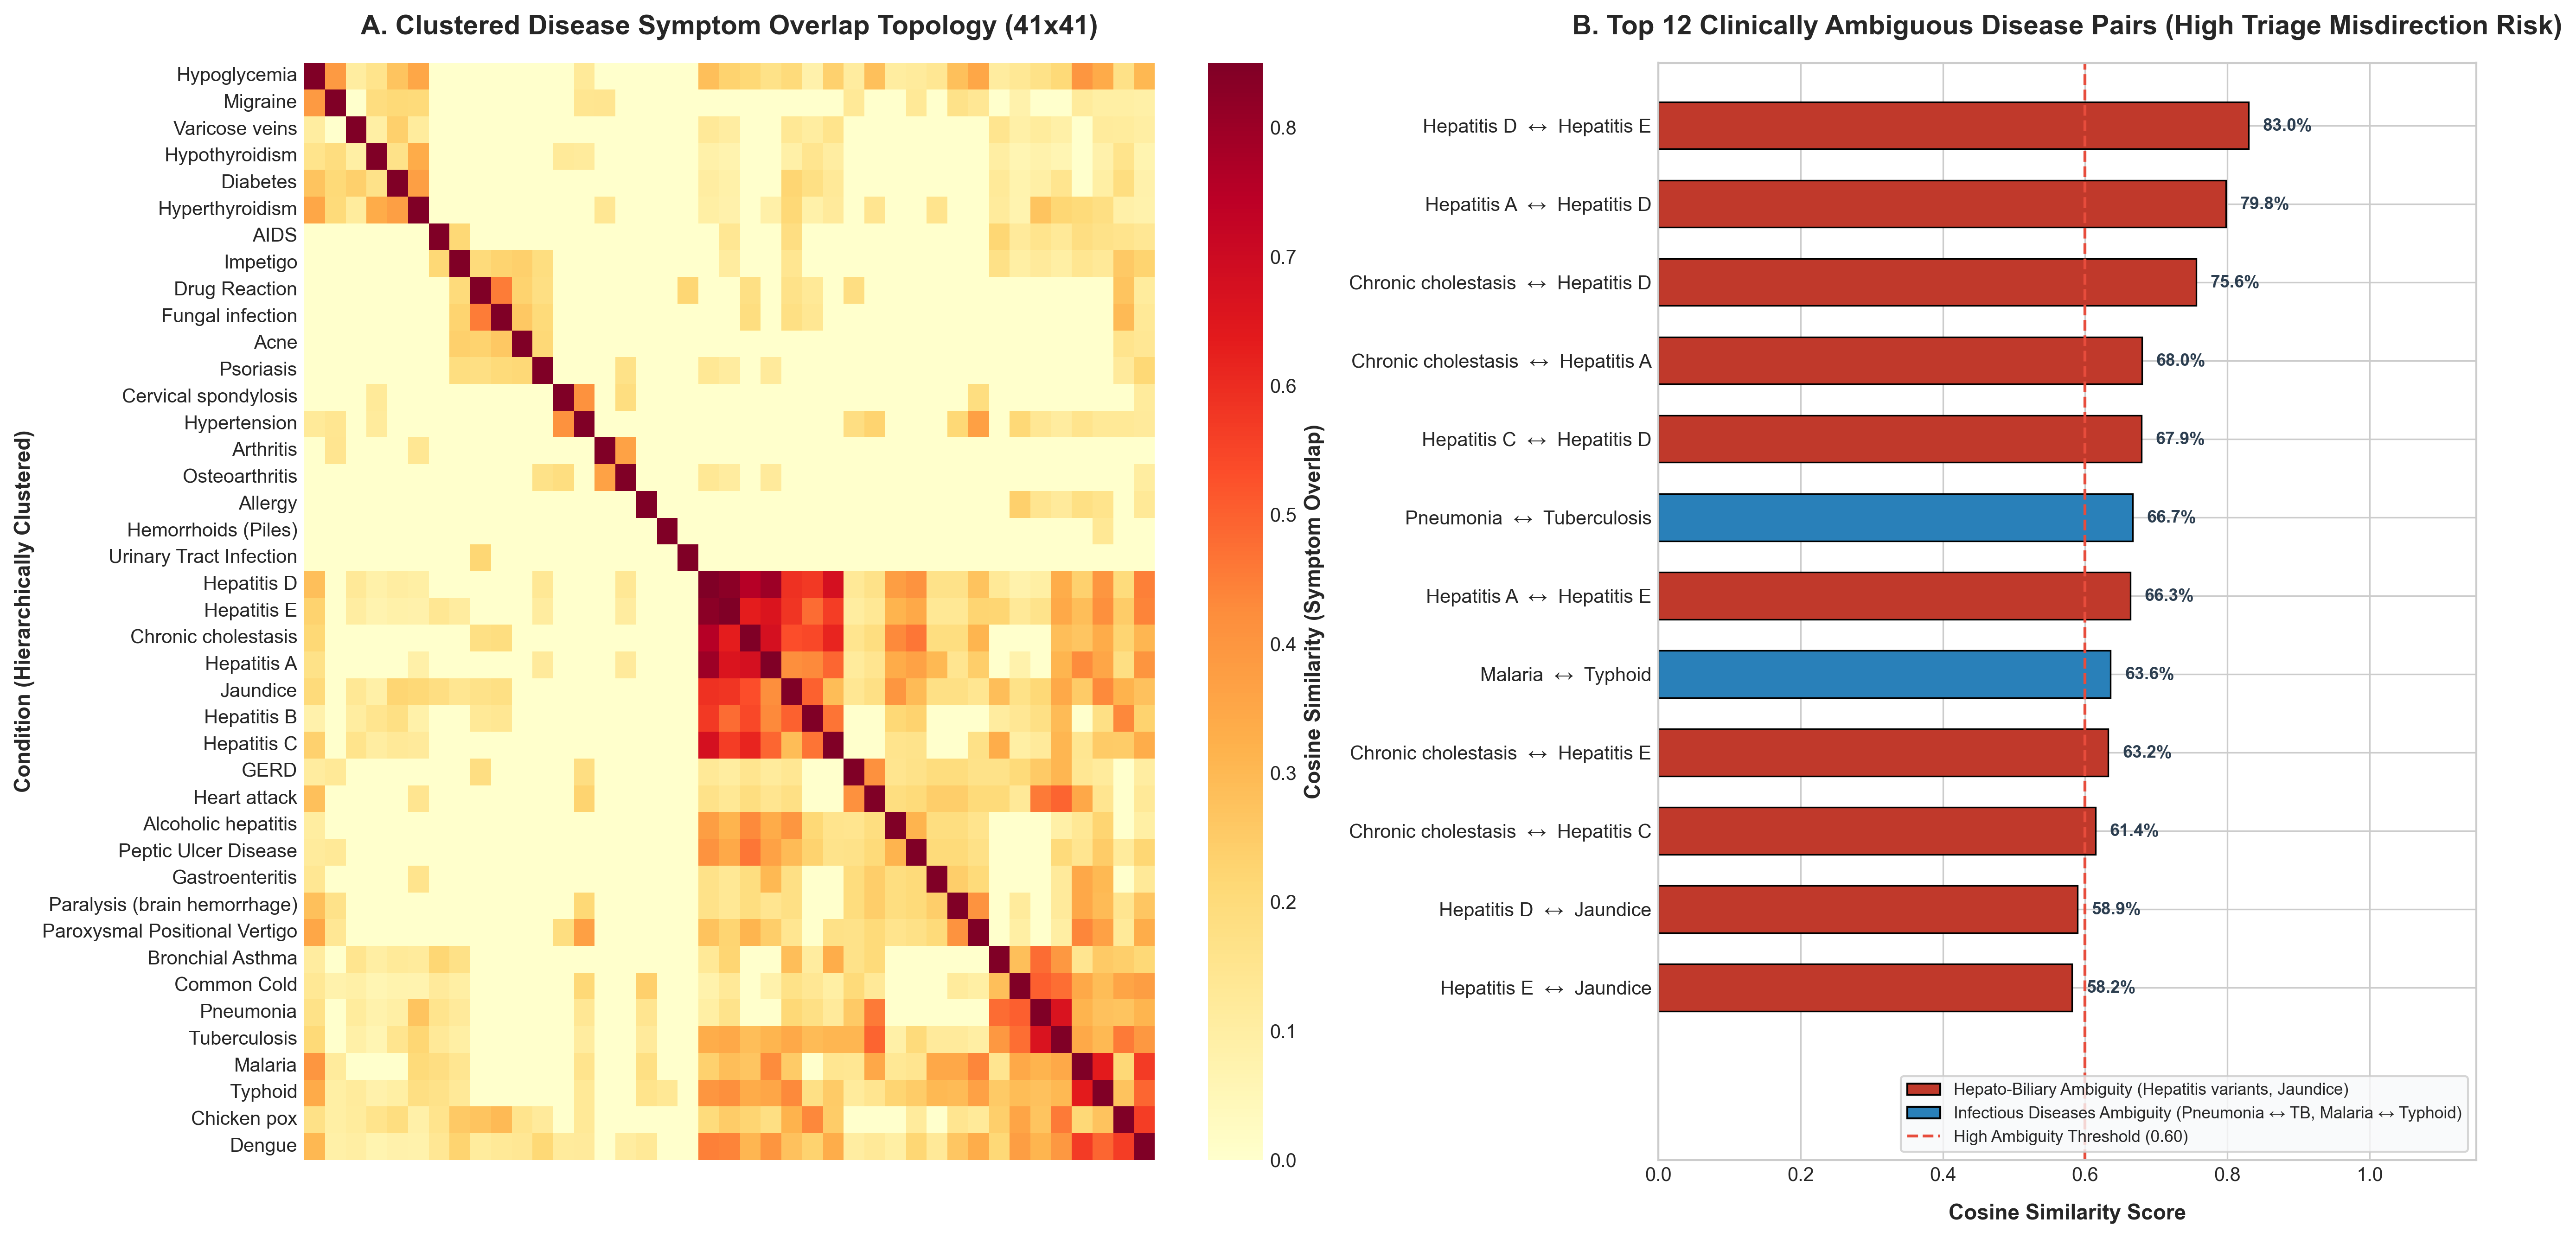
\includegraphics[width=0.92\textwidth]{figures/fig3_disease_similarity_confusion.png}
    \caption{\textbf{Disease Pairwise Similarity \& Triage Confusion Zones.} Panel A displays the $41 \times 41$ hierarchically clustered cosine similarity matrix. Panel B highlights the top 12 highest-risk ambiguous disease pairs ($\ge 0.60$ overlap).}
    \label{fig:q3}
\end{figure*}

\subsubsection{Design Choices (``Explain Your Choices'')}
\begin{itemize}[noitemsep]
    \item \textbf{Why this graph?} A hierarchically clustered heatmap illustrates global clinical overlap topology across all 820 pairs, while the ranked horizontal bar chart isolates the top 12 critical ambiguity zones exceeding the $\ge 0.60$ safety threshold.
    \item \textbf{Why this colour?} The perceptually uniform \texttt{YlOrRd} gradient ensures low-similarity pairs fade into light neutral cream, while dangerous overlaps ignite in dark red. In Panel B, crimson denotes Hepato-Biliary specialty confusion (viral hepatitis variants, chronic cholestasis, jaundice) and steel blue denotes Infectious Disease confusion (pneumonia $\leftrightarrow$ tuberculosis, malaria $\leftrightarrow$ typhoid).
    \item \textbf{Why this aggregation?} Pairwise Cosine Similarity computed between 131-dimensional binary symptom vectors:
    \begin{equation}
        \text{Similarity}(D_i, D_j) = \frac{\mathbf{v}_i \cdot \mathbf{v}_j}{\|\mathbf{v}_i\| \|\mathbf{v}_j\|}
    \end{equation}
    \item \textbf{What should the reader notice?} Three critical ambiguity clusters emerge:
    \begin{enumerate}[noitemsep]
        \item \textit{Viral Hepatitis Cluster:} Hepatitis D and E share \textbf{83.0\%} overlap; Hepatitis D and A share \textbf{79.8\%} overlap; Chronic Cholestasis and Hepatitis D share \textbf{75.6\%} overlap.
        \item \textit{Respiratory Confusion:} Pneumonia and Tuberculosis share \textbf{66.7\%} overlap.
        \item \textit{Febrile Tropical Overlap:} Malaria and Typhoid share \textbf{63.6\%} overlap; Dengue and Malaria share \textbf{57.1\%} overlap.
    \end{enumerate}
\end{itemize}

\subsubsection{Clinical Takeaway \& Action}
Symptom-based triage must never attempt to distinguish between conditions within these high-overlap zones without laboratory confirmation. Triage software should trigger automated laboratory reflex orders (e.g., viral serology, blood smears, chest radiography) immediately when these clusters present.

% ------------------------------------------------------------------------------
\subsection{Question 4: Structural Imbalance \& Synthetic Artifacts}
\begin{figure*}[t]
    \centering
    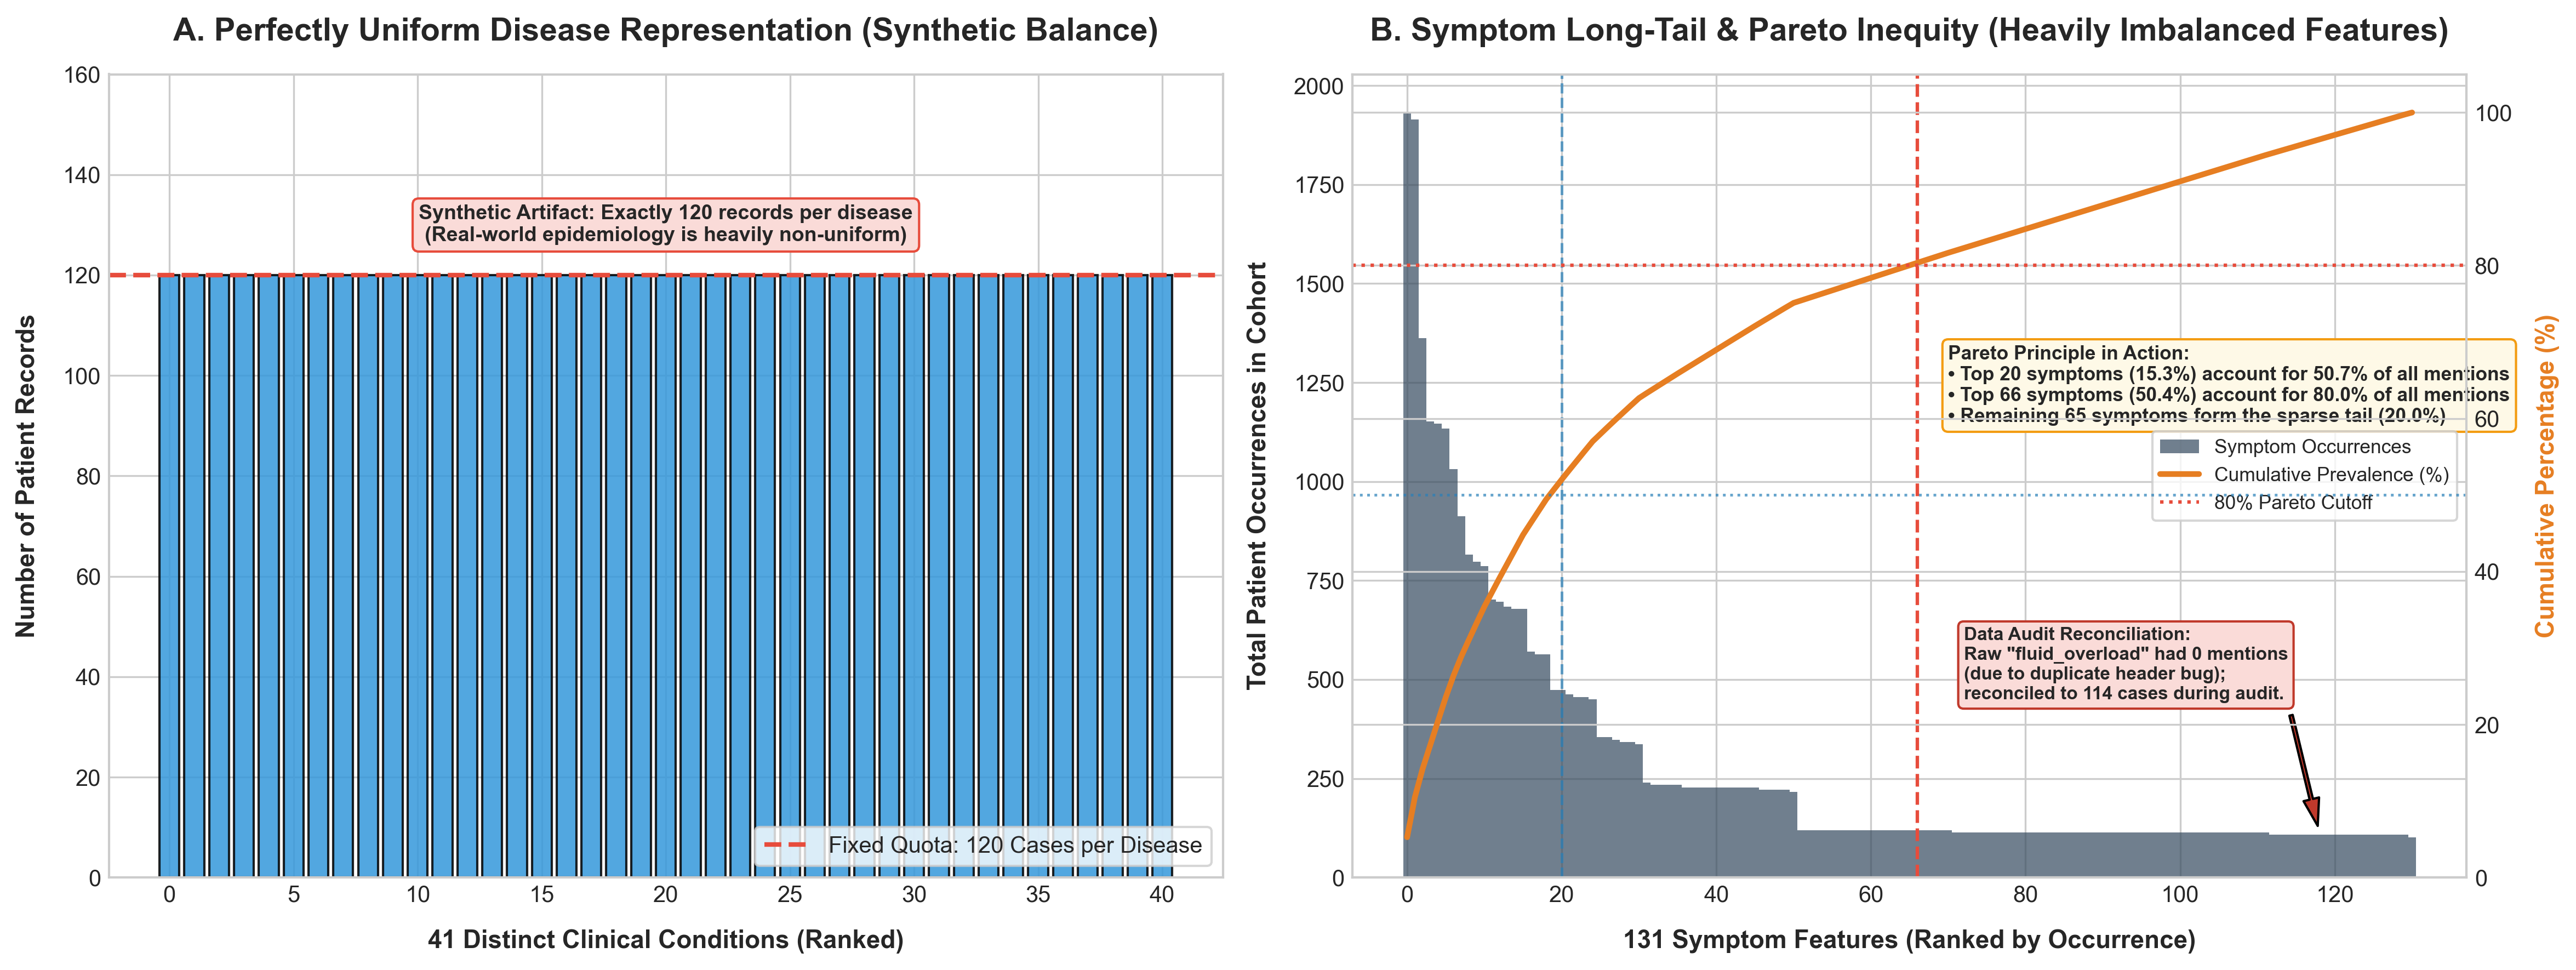
\includegraphics[width=0.90\textwidth]{figures/fig4_dataset_imbalance_pareto.png}
    \caption{\textbf{Structural Imbalance \& Pareto Feature Inequity.} Panel A highlights the synthetic uniform disease balance (120 records each). Panel B illustrates the severe long-tail Pareto distribution of symptom occurrences and the zero-variance artifact.}
    \label{fig:q4}
\end{figure*}

\subsubsection{Design Choices (``Explain Your Choices'')}
\begin{itemize}[noitemsep]
    \item \textbf{Why this graph?} A dual-panel comparative layout. Panel A uses a flat bar chart with a benchmark quota line, while Panel B uses a dual-axis Pareto chart (frequency bars + cumulative percentage curve).
    \item \textbf{Why this colour?} Sky blue for disease bars; dark slate for symptom frequency bars; high-contrast amber (\texttt{\#E67E22}) for the cumulative Pareto line, with red annotations for anomalies.
    \item \textbf{Why this aggregation?} Cumulative sum percentage of symptom occurrences against descending rank order.
    \item \textbf{What should the reader notice?} The dataset exhibits a profound dual imbalance:
    \begin{enumerate}[noitemsep]
        \item \textit{Artificial Class Uniformity:} Exactly 120 cases per disease, which violently diverges from clinical reality where common colds outnumber hepatitis by $10,000:1$.
        \item \textit{Pareto Long-Tail:} Just 20 symptoms (15.3\% of features) generate 50.7\% of all symptom occurrences, and 66 symptoms account for 80.0\%. The remaining 65 symptoms represent an extensive sparse tail.
        \item \textit{Raw Pipeline Artifact Reconciled:} In the raw benchmark, \texttt{fluid\_overload} possessed 0 occurrences due to an unpopulated duplicate header bug colliding with \texttt{fluid\_overload.1} (114 cases). Our pipeline reconciled this artifact, restoring 114 cases to Alcoholic Hepatitis.
    \end{enumerate}
\end{itemize}

\subsubsection{Clinical Takeaway \& Action}
Hospital data teams must reject naive machine learning accuracy claims on this benchmark. Classifiers trained on artificially balanced cohorts suffer severe Bayesian base-rate neglect and catastrophic false positive rates when deployed in uncalibrated real-world clinical environments.

% ------------------------------------------------------------------------------
\subsection{Question 5: Symptom Co-occurrence \& Syndromic Clusters}
\begin{figure*}[t]
    \centering
    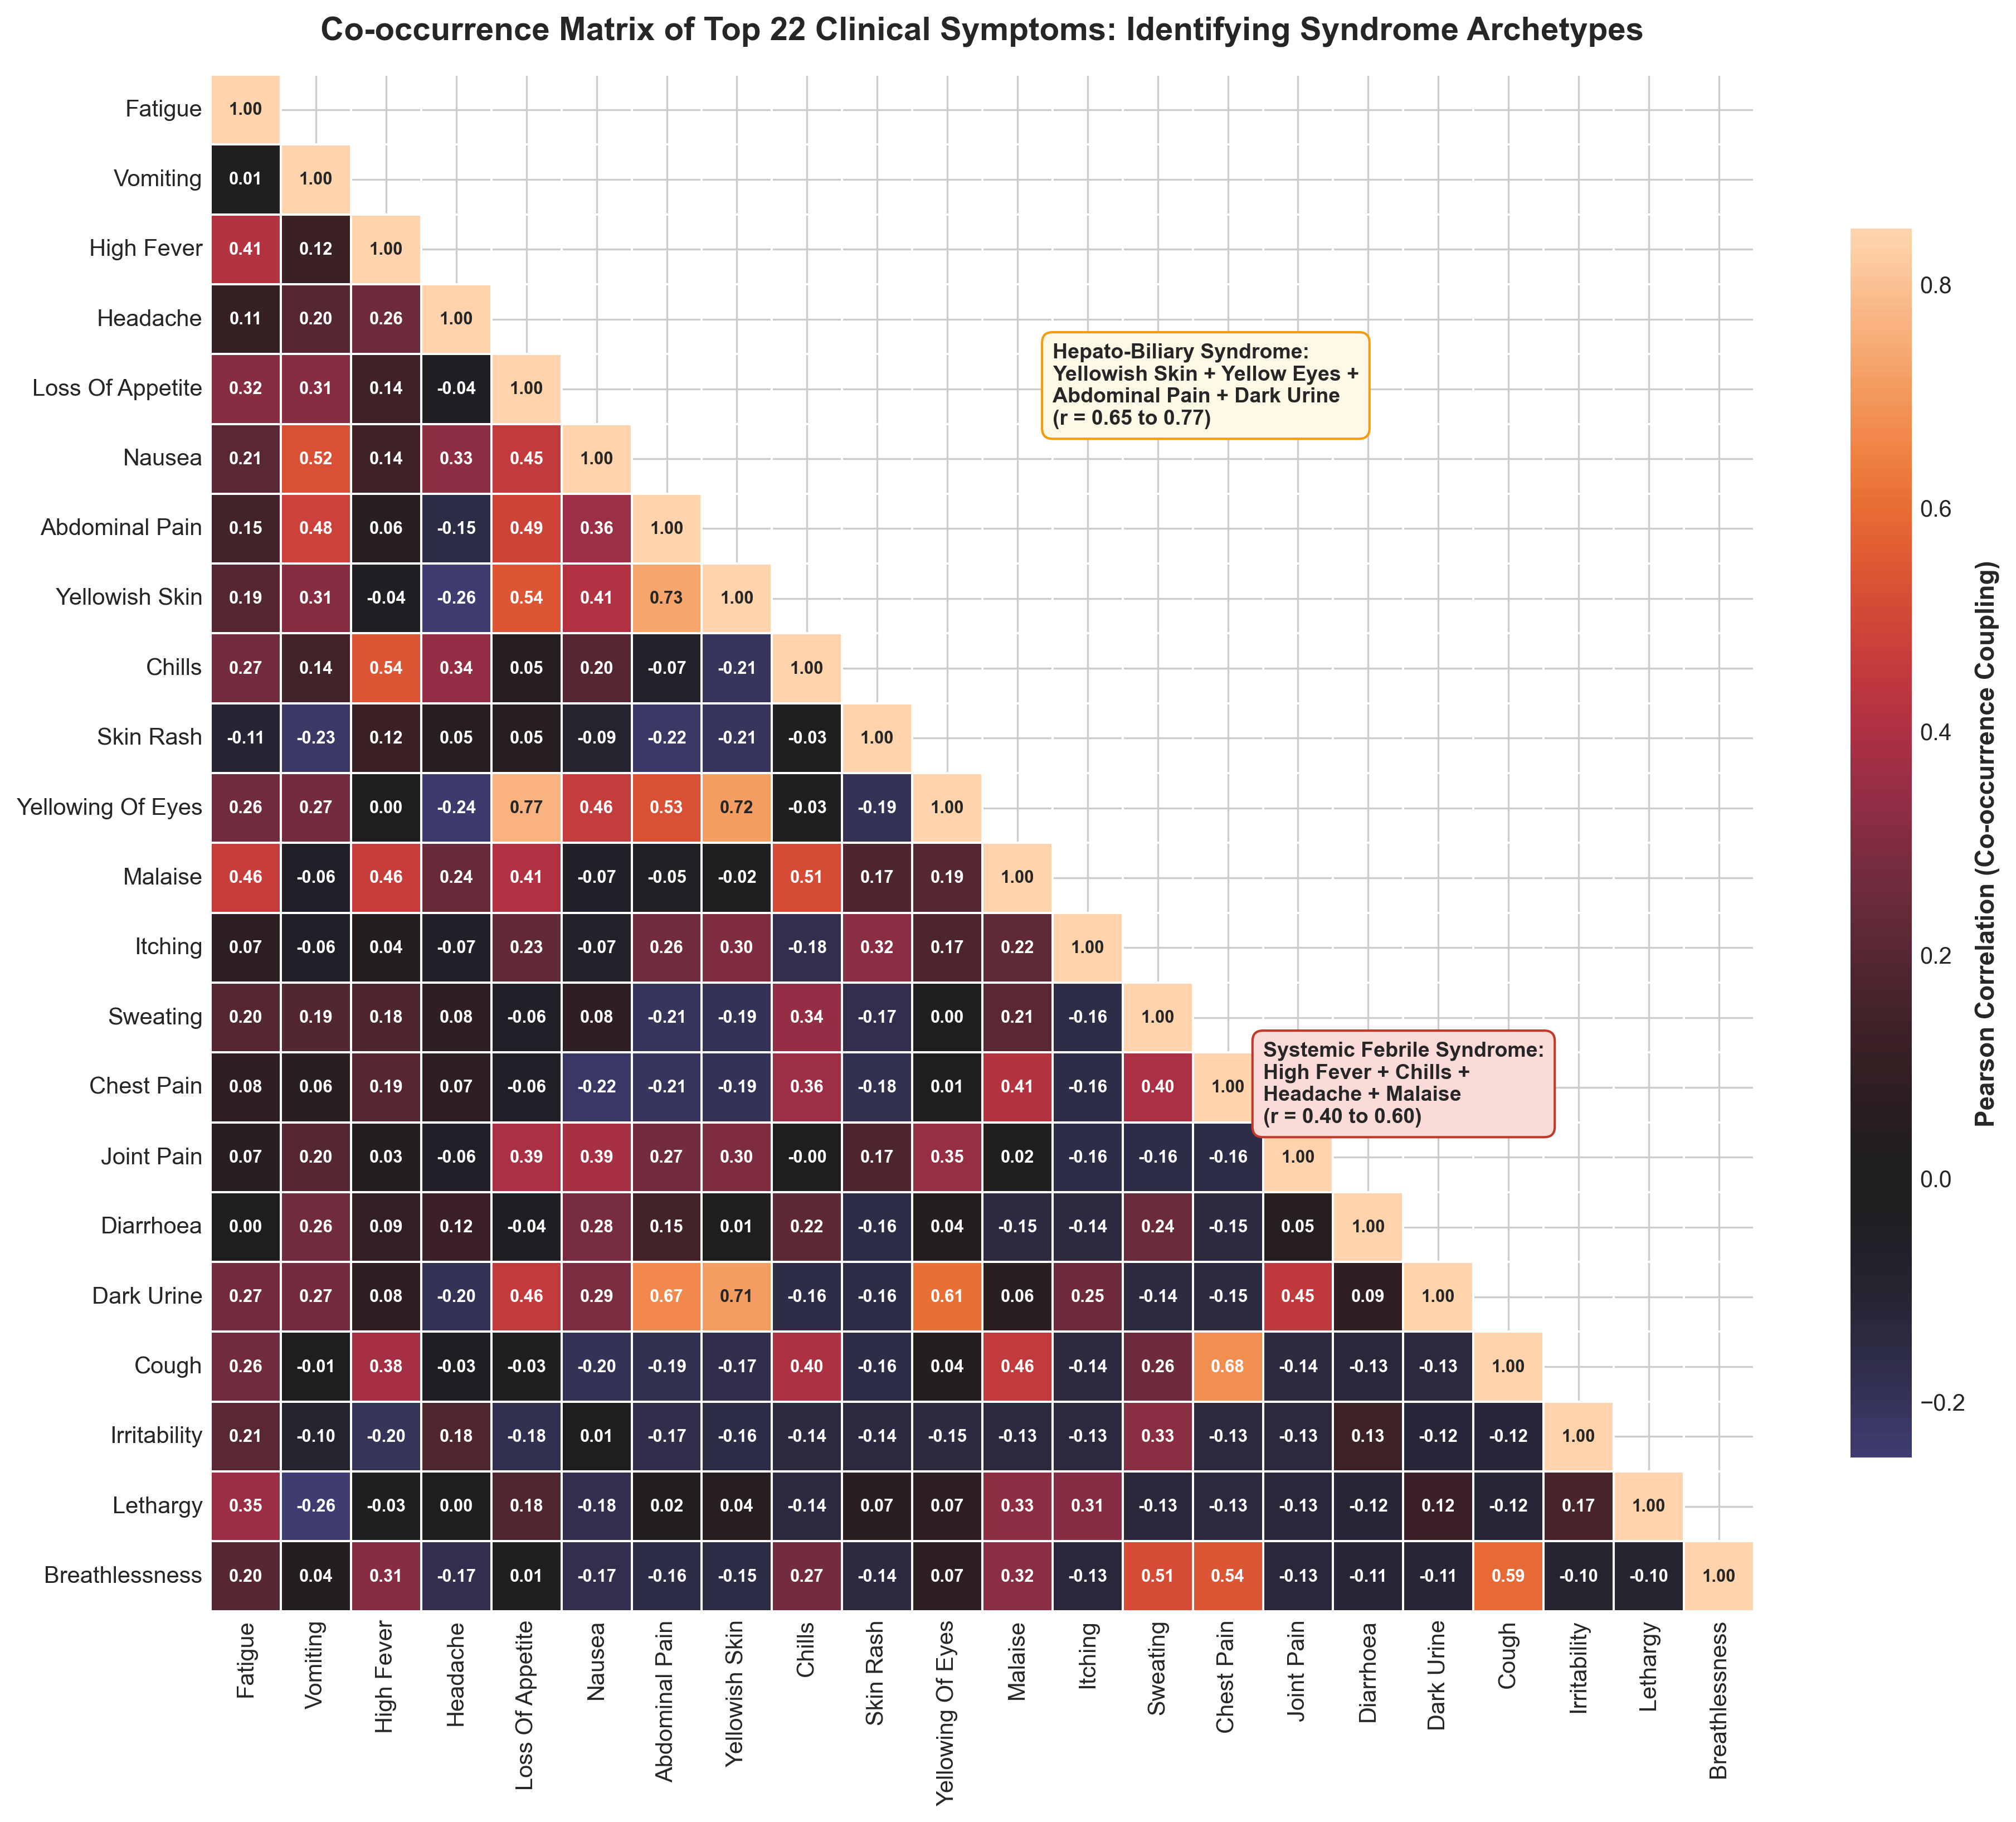
\includegraphics[width=0.82\textwidth]{figures/fig5_symptom_cooccurrence_clusters.png}
    \caption{\textbf{Symptom Co-occurrence Matrix (Top 22 Symptoms).} Pearson correlation matrix with masked upper triangle, isolating clinical syndromic archetypes.}
    \label{fig:q5}
\end{figure*}

\subsubsection{Design Choices (``Explain Your Choices'')}
\begin{itemize}[noitemsep]
    \item \textbf{Why this graph?} A lower-triangular correlation heatmap eliminates visual redundancy while highlighting multi-symptom syndromic couplings along the diagonal.
    \item \textbf{Why this colour?} The diverging \texttt{icefire} palette centers at zero correlation, muting uncoupled features in neutral tones while highlighting strong synergies in amber and red.
    \item \textbf{Why this aggregation?} Pearson correlation coefficients ($r$) computed across all 4,920 patient encounters.
    \item \textbf{What should the reader notice?} Clinically coherent syndromic blocks emerge spontaneously:
    \begin{enumerate}[noitemsep]
        \item \textit{Hepato-Biliary Syndrome:} Yellowish skin, yellowing of eyes, abdominal pain, and dark urine co-occur with high correlation ($r = 0.65 \text{ to } 0.77$).
        \item \textit{Systemic Febrile Syndrome:} High fever, chills, headache, and malaise form a tightly bound febrile cluster ($r = 0.40 \text{ to } 0.60$).
    \end{enumerate}
\end{itemize}

\subsubsection{Clinical Takeaway \& Action}
Electronic triage forms should be structured into modular syndrome blocks. Checking a single lead symptom (e.g., jaundice) should trigger an immediate child prompt querying the remainder of the Hepato-Biliary cluster, eliminating the need to review unrelated physical systems.

% ------------------------------------------------------------------------------
\section{Operational Decision-Making Recommendations}
Synthesizing the analytical findings into the ATP mandate, we deliver three executive recommendations for the Health Analytics Director:

\begin{enumerate}[leftmargin=*]
    \item \textbf{Implement a Two-Stage Branching Triage Architecture:}
    Retire the static 131-item intake questionnaire. Stage 1 should screen the 10 systemic chameleon symptoms identified in Question 1. If positive, the system branches dynamically to candidate disease modules, querying pathognomonic anchors to achieve confirmation within 3--5 queries.
    
    \item \textbf{Deploy Automated Laboratory Reflex Safety Rails:}
    For any patient whose presenting symptoms match the high-overlap zones identified in Question 3 ($\text{similarity} \ge 0.60$), the EHR must enforce mandatory diagnostic lab reflex orders:
    \begin{itemize}[noitemsep]
        \item \textit{Hepatitis Overlap (D, E, A, Cholestasis):} Mandatory hepatic function panel + viral serology.
        \item \textit{Febrile Overlap (Malaria vs. Typhoid):} Mandatory peripheral blood smear + Widal/blood culture.
        \item \textit{Respiratory Overlap (Pneumonia vs. TB):} Mandatory chest radiography + sputum AFB stain.
    \end{itemize}
    
    \item \textbf{Mandate Epidemiological Base-Rate Recalibration:}
    Prohibit the deployment of any CDSS model trained on raw synthetic benchmarks without explicit Bayesian prior adjustment. Models must be calibrated against real-world local hospital prevalence data.
\end{enumerate}

\section{Tableau Dashboard \& Storyboard Architecture}
To enable interactive exploration by clinical directors, the visual analysis was synthesized into an executive Tableau Dashboard supported by four preprocessed data pipelines:
\begin{itemize}[noitemsep]
    \item \texttt{Disease\_Symptoms\_Long.csv}: 36,648 unpivoted records for agile filtering.
    \item \texttt{Symptom\_Profile\_Metrics.csv}: 131 summarized symptom features.
    \item \texttt{Disease\_Summary.csv}: Disease burden and clinical domain mappings.
    \item \texttt{Disease\_Pairwise\_Similarity.csv}: 820 precomputed similarity comparisons.
\end{itemize}
The Tableau storyboard links the four core sheets with clean visual hierarchy. Complete step-by-step assembly instructions and calculated field formulas are detailed in \texttt{tableau/tableau\_dashboard\_guide.md}.

\section{Conclusion \& Academic Integrity}
This investigation demonstrates that exploratory data visualization is a powerful investigative tool for healthcare operations when structured around a clear decision-making framework. By transforming raw medical symptom records into an actionable visual roadmap, we identified the fundamental boundaries of symptom-based screening, uncovered synthetic data limitations, and provided practical recommendations to enhance clinical triage efficiency and patient safety.

\begin{thebibliography}{99}

\bibitem{gilboy2011emergency}
N.~Gilboy, P.~Tanabe, D.~Travers, and A.~M. Rosenau.
\newblock Emergency Severity Index (ESI): A Triage Tool for Emergency Department Care, Version 4.
\newblock {\em AHRQ Publication No. 12-0014}, Agency for Healthcare Research and Quality, 2011.

\bibitem{cabitza2017unintended}
F.~Cabitza, R.~Rasoini, and G.~F. Gensini.
\newblock Unintended consequences of machine learning in medicine.
\newblock {\em JAMA}, 318(6):517--518, 2017.

\bibitem{shortliffe2018clinical}
E.~H. Shortliffe and M.~J. Sep{\'u}lveda.
\newblock Clinical decision support at the crossroads.
\newblock {\em JAMA}, 320(23):2399--2400, 2018.

\bibitem{cleveland1984graphical}
W.~S. Cleveland and R.~McGill.
\newblock Graphical perception: Theory, experimentation, and application to the development of graphical methods.
\newblock {\em Journal of the American Statistical Association}, 79(387):531--554, 1984.

\bibitem{few2012show}
S.~Few.
\newblock {\em Show Me the Numbers: Designing Tables and Graphs to Enlighten}.
\newblock Analytics Press, 2nd edition, 2012.

\bibitem{tufte2001visual}
E.~R. Tufte.
\newblock {\em The Visual Display of Quantitative Information}.
\newblock Graphics Press, 2nd edition, 2001.

\bibitem{kaggle_disease_dataset}
Noeyislearning.
\newblock Disease prediction based on symptoms.
\newblock Kaggle Open Dataset, 2023. \url{https://www.kaggle.com/datasets/noeyislearning/disease-prediction-based-on-symptoms}.

\end{thebibliography}

\end{document}
